\section*{Exercise 5}

\subsection*{Exercise 5 (4)}
\href{http://v1.probmods.org/conditioning.html#exercises}{Probabilistic Models of Cognition - Exercise 4}

\paragraph{Solution}
The developed program is written in Church and it is memorized in the file \textit{exercise\_5.rkt}. This file is a Racket file, but 
the code is written in Church, so to be executed it is necessary to use a Church interpreter.

The answers to the questions are written below:
\begin{itemize}
    \item[A.] The posterior probability $P(h\;|\;\text{win})$ is the conditional probability that the machine randomly gives to Bob
        a specific letter knowing that Bob has won. In particular, the fact that Bob has won is called \textit{evidence} and it is all
        we kwnow. The posterior probability can be computed by the Bayes' theorem by knowing: \textit{(i)} the conditional 
        probability $P(win\;|\;\text{h})$ (or \textit{likelihood}); \textit{(ii)} the prior probability $P(h)$ and 
        \textit{(iii)} the marginal probability $P(win)$.
        In particular it is proven that:
        \[ P(h\;|\;\text{win}) = \frac{P(win\;|\;\text{h}) \cdot P(h)}{P(win)}\]
    
    \item[B.] The probability $P(h\;|\;\text{win})$ has been manually computed for each hypothesis with Excel. First of all, the
        \textit{likelihood} has been computed by using the following formula: $P(win\;|\;\text{h}) = 1/Q(h)^{2}$ where $Q(h)$ is
        the position of the letter in the alphabet. Then the numerator of the formula of the Bayes' theorem is computed.
        To compute the marginal probability $P(win)$ the following formula has be used:
        \[ P(win) = \sum_{h} P(win\;|\;\text{h}) \cdot P(h)\]
        After that the posterior probability has been computed for each hypothesis by using the Bayes' theorem and the results are shown
        in Table~\ref{tab:casino-game}.
        \begin{table}[H]
            \centering
            \begin{minipage}{.4\linewidth}
                \centering
                \begin{tabular}{c c}
                    \hline
                    \textbf{Letter} & $P(h\;|\;\text{win})$ \\
                    \hline
                    \textit{a} & $0.2755$ \\
                    \textit{b} & $0.3237$ \\
                    \textit{c} & $0.1439$ \\
                    \textit{d} & $0.0809$ \\
                    \textit{e} & $0.0110$ \\
                    \textit{f} & $0.0360$ \\
                    \textit{g} & $0.0264$ \\
                    \textit{h} & $0.0202$ \\
                    \textit{i} & $0.0034$ \\
                    \textit{j} & $0.0130$ \\
                    \textit{k} & $0.0107$ \\
                    \textit{l} & $0.0090$ \\
                    \textit{m} & $0.0077$ \\
                    \hline
                \end{tabular}
            \end{minipage}
            \begin{minipage}{.4\linewidth}
                \centering
                \begin{tabular}{c c}
                    \hline
                    \textbf{Letter} & $P(h\;|\;\text{win})$ \\
                    \hline
                    \textit{n} & $0.0066$ \\
                    \textit{o} & $0.0012$ \\
                    \textit{p} & $0.0051$ \\
                    \textit{q} & $0.0045$ \\
                    \textit{r} & $0.0040$ \\
                    \textit{s} & $0.0036$ \\
                    \textit{t} & $0.0032$ \\
                    \textit{u} & $0.0006$ \\
                    \textit{v} & $0.0027$ \\
                    \textit{w} & $0.0025$ \\
                    \textit{x} & $0.0022$ \\
                    \textit{y} & $0.0005$ \\
                    \textit{z} & $0.0019$ \\
                    \hline
                \end{tabular}
            \end{minipage}
            
            \caption{Manually computed posterior probability $P(h\;|\;\text{win})$ for each hypothesis}
            \label{tab:casino-game}
        \end{table}
    \item[C.] The procedure \texttt{my-list-index} takes in input 3 parameters: \textit{(i)} \texttt{needle} that is an object, 
        which can be a number, a list, a quoted symbol or something else; \textit{(ii)} \texttt{haystack} that is a list containing zero 
        or more elements; \textit{(iii)} \texttt{counter} that is a number. 
        The procedure then returns \texttt{\textquotesingle error} if \texttt{needle} is not present in \texttt{haystack}, otherwise it returns the
        third argument (i.e. the number) incremented by the position of the \texttt{needle} in the list; the position is considered to be
        zero-based, so the first element of the list has index $0$, therefore if the \texttt{needle} is in the first position of the list 
        \texttt{haystack}, then the \texttt{counter} is not incremented. If the \texttt{counter} has value $0$ when the procedure is 
        called, then the procedure returns the position zero-based of the \texttt{needle} (if present), instead, if the value of the
        \texttt{counter} is $1$, then the procedure returns the position one-based of the \texttt{needle} in the \texttt{haystack}.
    
    \item[D.] The procedure \texttt{multinomial} takes in input two lists: the first one is a list of possible outcomes, whereas the 
        second one is the list of the weights associated to the outcomes in the first list. In particular, the higher is the weight
        of one element relative to the weights of the other elements, the higher is the probability to get that specific
        element. Indeed, the probability to get the element at a specific position $i$ is given by the following formula:
        \[ P(e_{i}) = \frac{weight(e_{i})}{\sum_{j} weight(e_{j})} \]
        where $e_{i}$ and $e_{j}$ are the elements of the first list and the function \textit{weight} returns the weight associated
        to the element (i.e. the weight of the second list which is in the same position of the element in the first list).

        To implement the distribution of Table~\ref{tab:casino-game} with the procedure \texttt{multinomial}, two lists have been
        defined: \textit{(i)} \texttt{x} which contains all the possible outcomes and \textit{(ii)} \texttt{x-weights} which contains
        the weight of the elements of the first list. An alternative definition of the list \texttt{x-weights} is provided in order to
        prove that the formula previously defined holds.
        Then a simple model is defined: it simply returns a value of the first list according to the probabilities defined by the
        second list.
        \begin{lstlisting}[caption={Program which implements with \texttt{multinomial} the distribution of Table~\ref{tab:casino-game}}, 
            captionpos=b, label={lst:casino-game-d}]
; definition of the possible outcomes
(define x '(red blue green black))

; definition of the probability for each outcome
(define x-weights '(0.5 0.05 0.4 0.05))

; equivalent definition of the x-weights
; (define x-weights '(5 0.5 4 0.5))

; definition of a model which represents 
; the distribution given in the exercise
(define (model)
  (multinomial x x-weights))

; visualization of the results
(hist (repeat 10000 model))
        \end{lstlisting}
        Finally some samples are generated in order to show that the implemented distribution is equivalent to the distribution defined
        in Table~\ref{tab:casino-game}. The results are shown in Figure~\ref{fig:casino-game-d}.
        \begin{figure}[ht!]
            \centering
            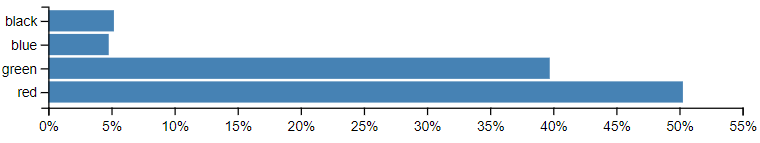
\includegraphics[width=\linewidth]{images/5.4.d.png}
            \caption{
                Distribution of the samples generated with the code in Listing~\ref{lst:casino-game-d}.
            }
            \label{fig:casino-game-d}
        \end{figure}
    \item[E.] The code is completed as shown in Listing \ref{lst:casino-game-e}, in particular it is reported only the definition of
        \texttt{distribution} because the other parts remain the same.
        \begin{lstlisting}[caption={Definition of \texttt{distribution} in order to compute $P(h\;|\;\text{win})$.}, captionpos=b,
            label={lst:casino-game-e}]
(define distribution
  (enumeration-query
   (define my-letter 
     (multinomial letters letter-probabilities))

   (define my-position (get-position my-letter))
   (define my-win-probability 
     (/ 1.0 (* my-position my-position)))
   (define win? (if (equal? my-letter 'a) 
                    #t 
                    (flip my-win-probability)))

   ; query to get the probability P(h | win)
   my-letter

   ; query to get the probabilities P(vowel | win)
   ; and P(consonant | win)
   ; (if (vowel? my-letter) 'vowel 'consonant) 

   ;; condition
   win?
   ))
        \end{lstlisting}
        The approximate distribution is shown in Figure~\ref{fig:casino-game-e}. It is possible to observe that the computed
        probabilities are similar to the probabilities manually computed and that the letter with higher posterior probability
        is the letter \textit{b}. This means that when we know that Bob has won, then it is more likely that he has received the
        letter \textit{b} by the machine.
        \begin{figure}[ht!]
            \centering
            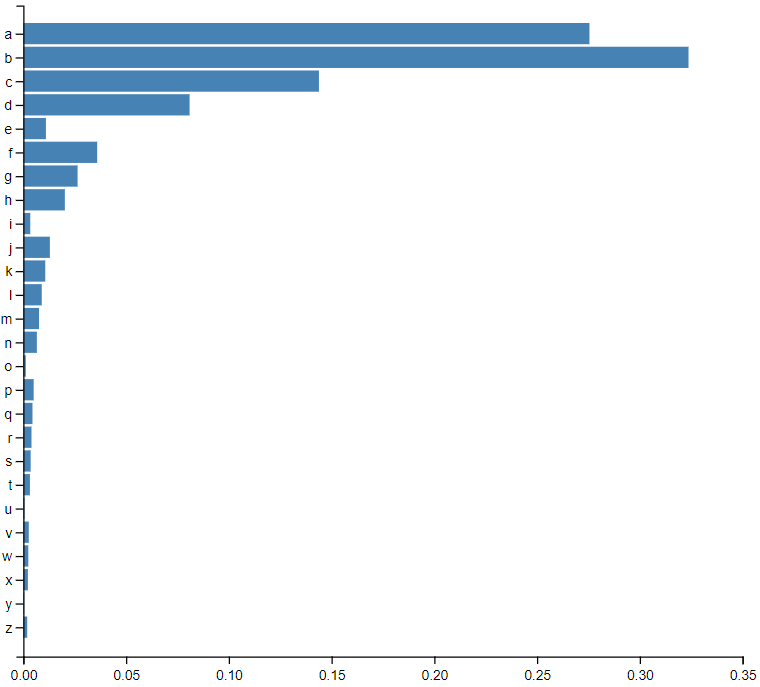
\includegraphics[width=7cm]{images/5.4.e.png}
            \caption{
                Approximate distribution of posterior probability $P(h\;|\;\text{win})$ through the code in 
                Listing~\ref{lst:casino-game-e}.
            }
            \label{fig:casino-game-e}
        \end{figure}
    \item[F.] To compute the posterior probabilities $P(vowel\;|\;\text{win})$ and $P(consonant\;|\;\text{win})$ it is sufficient to
        replace the query part of the code in Listing~\ref{lst:casino-game-e} with the following piece of code:
        \begin{lstlisting}[caption={Code to be put in place of \texttt{my-letter} in Listing~\ref{lst:casino-game-e}}, captionpos=b]
(if (vowel? my-letter) 'vowel 'consonant) 
        \end{lstlisting}
        The result is that the program now computes the probability to get a \textit{vowel} or a \textit{consonant} given the evidence
        that Bob has won. We can observe in Figure~\ref{fig:casino-game-f} that it is more likely that Bob has received a consonant
        instead of a vowel.
        \begin{figure}[ht!]
            \centering
            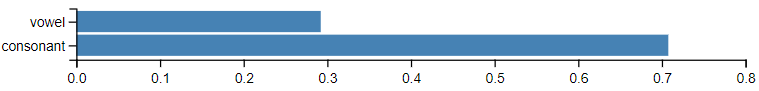
\includegraphics[width=\linewidth]{images/5.4.f.png}
            \caption{
                Approximate distribution of probabilities $P(vowel\;|\;\text{win})$ and $P(consonant\;|\;\text{win})$.
            }
            \label{fig:casino-game-f}
        \end{figure}
    \item[G.] With the mathematical notation the computation is made without taking into account all the probability tree, but it is
        sufficient to apply the Bayes' theorem in order to compute the posterior probabilities. Instead, by using the Church program
        the computation is completely automatic and the only thing to do is to define the prior probabilities and then to define the
        query and the evidence. The disadvantage of the Church computation is that the interpreter has to evaluate all the paths in
        the probability tree, so it can be used only when the domain of interest is limited and when the query is not too complex.
\end{itemize}